\documentclass{beamer}
\usepackage{ctex}
\usetheme{Madrid}
\usepackage{ulem}
\usepackage{makecell}
\usepackage{multirow}
\usepackage{subcaption}

\title{某退役选手的文化课经历}
\author{caeious}
\date{2024.2.17}

\begin{document}

% Title page frame
\begin{frame}
    \titlepage
\end{frame}

\begin{frame}{自我介绍}
\begin{itemize}
    \item 第 39 届全国青少年信息学奥林匹克竞赛(NOI2022)银牌
    \item 2021 年高中数学联赛“真省一”
    \item 2023 年高考省 689 名
    \item 现就读于清华大学致理书院信息与计算科学专业
\end{itemize}
\end{frame}

\begin{frame}{摘要}
    \tableofcontents[hideallsubsections]
    \begin{alertblock}{注意时效性!}
        这里的内容均针对江苏省 2023 年的情况。务必查看您升学对应年份新发布的招生简章等资料。
    \end{alertblock}
\end{frame}
\AtBeginSection[]
{
\begin{frame}{摘要}
    \tableofcontents[currentsection]
\end{frame}
}

\section{政策指北}

\subsection{上学方式一览}
\begin{frame}{上学方式一览}
    \begin{itemize}
        \pause
        \item 保送
        \pause
        \item 高考裸分
        \pause
        \item 特殊项目:
        \begin{table}[h!]
            \centering
            \begin{tabular}{|c|c|c|}
              \hline
              学科 & 清华大学 & 北京大学 \\
              \hline
              \multirow{2}{*}{数学} & 丘成桐英才班 & \multirow{2}{*}{数学英才班} \\
              \cline{2-2}
              & 新领军 &\\ 
              \hline
              物理 & 攀登计划 & 卓越计划\\
              \hline
            \end{tabular}
            \label{tab:special projects}
        \end{table}
        \pause
        \item 综合评价
        \pause
        \item 强基计划
    \end{itemize}
\end{frame}

\subsection{综合评价}
\begin{frame}{综合评价}
    \begin{itemize}
        \pause
        \item 可报考范围:本省高校 和 中外合作办学
        \item 不同学校综合分计算方法、报考流程、考试内容等差别很大,具体见各高校招生简章
        \pause
        \begin{alertblock}{当心综评锁档}
            如果被多个途径录取,会遵照 \underline{强基 > 综评A类 > 裸分}投档,有时需要视估分放弃校测。
        \end{alertblock}
    \end{itemize}
\end{frame}

\subsection{强基计划}
\begin{frame}{强基计划}
    \begin{itemize}
        \pause
        \item 可报考范围:985 高校
        \item 限制转专业
        \item 全部具有保研资格(但还需要被导师录取,类似语言类保送资格考的“资格”)
        \item 综合高考和“校测”成绩录取
    \end{itemize}
\end{frame}

\section{清华强基的报考流程}

\subsection{报名}
\begin{frame}{报名/填写报名表}
    \begin{itemize}
        \pause
        \item 4月:招生简章公布,需要在\textbf{两个系统}上填报名信息。
        \pause
        \item 确保填在报名表上的内容真实且自己了解。
        \item 在此基础上,尽量不要留空白栏目。
        \pause
        \item “大中衔接”之类的获奖可以写在个人陈述里。
    \end{itemize}
\end{frame}

\begin{frame}{报名/志愿填报}
    \pause
    \begin{figure}[h!]
        \centering
        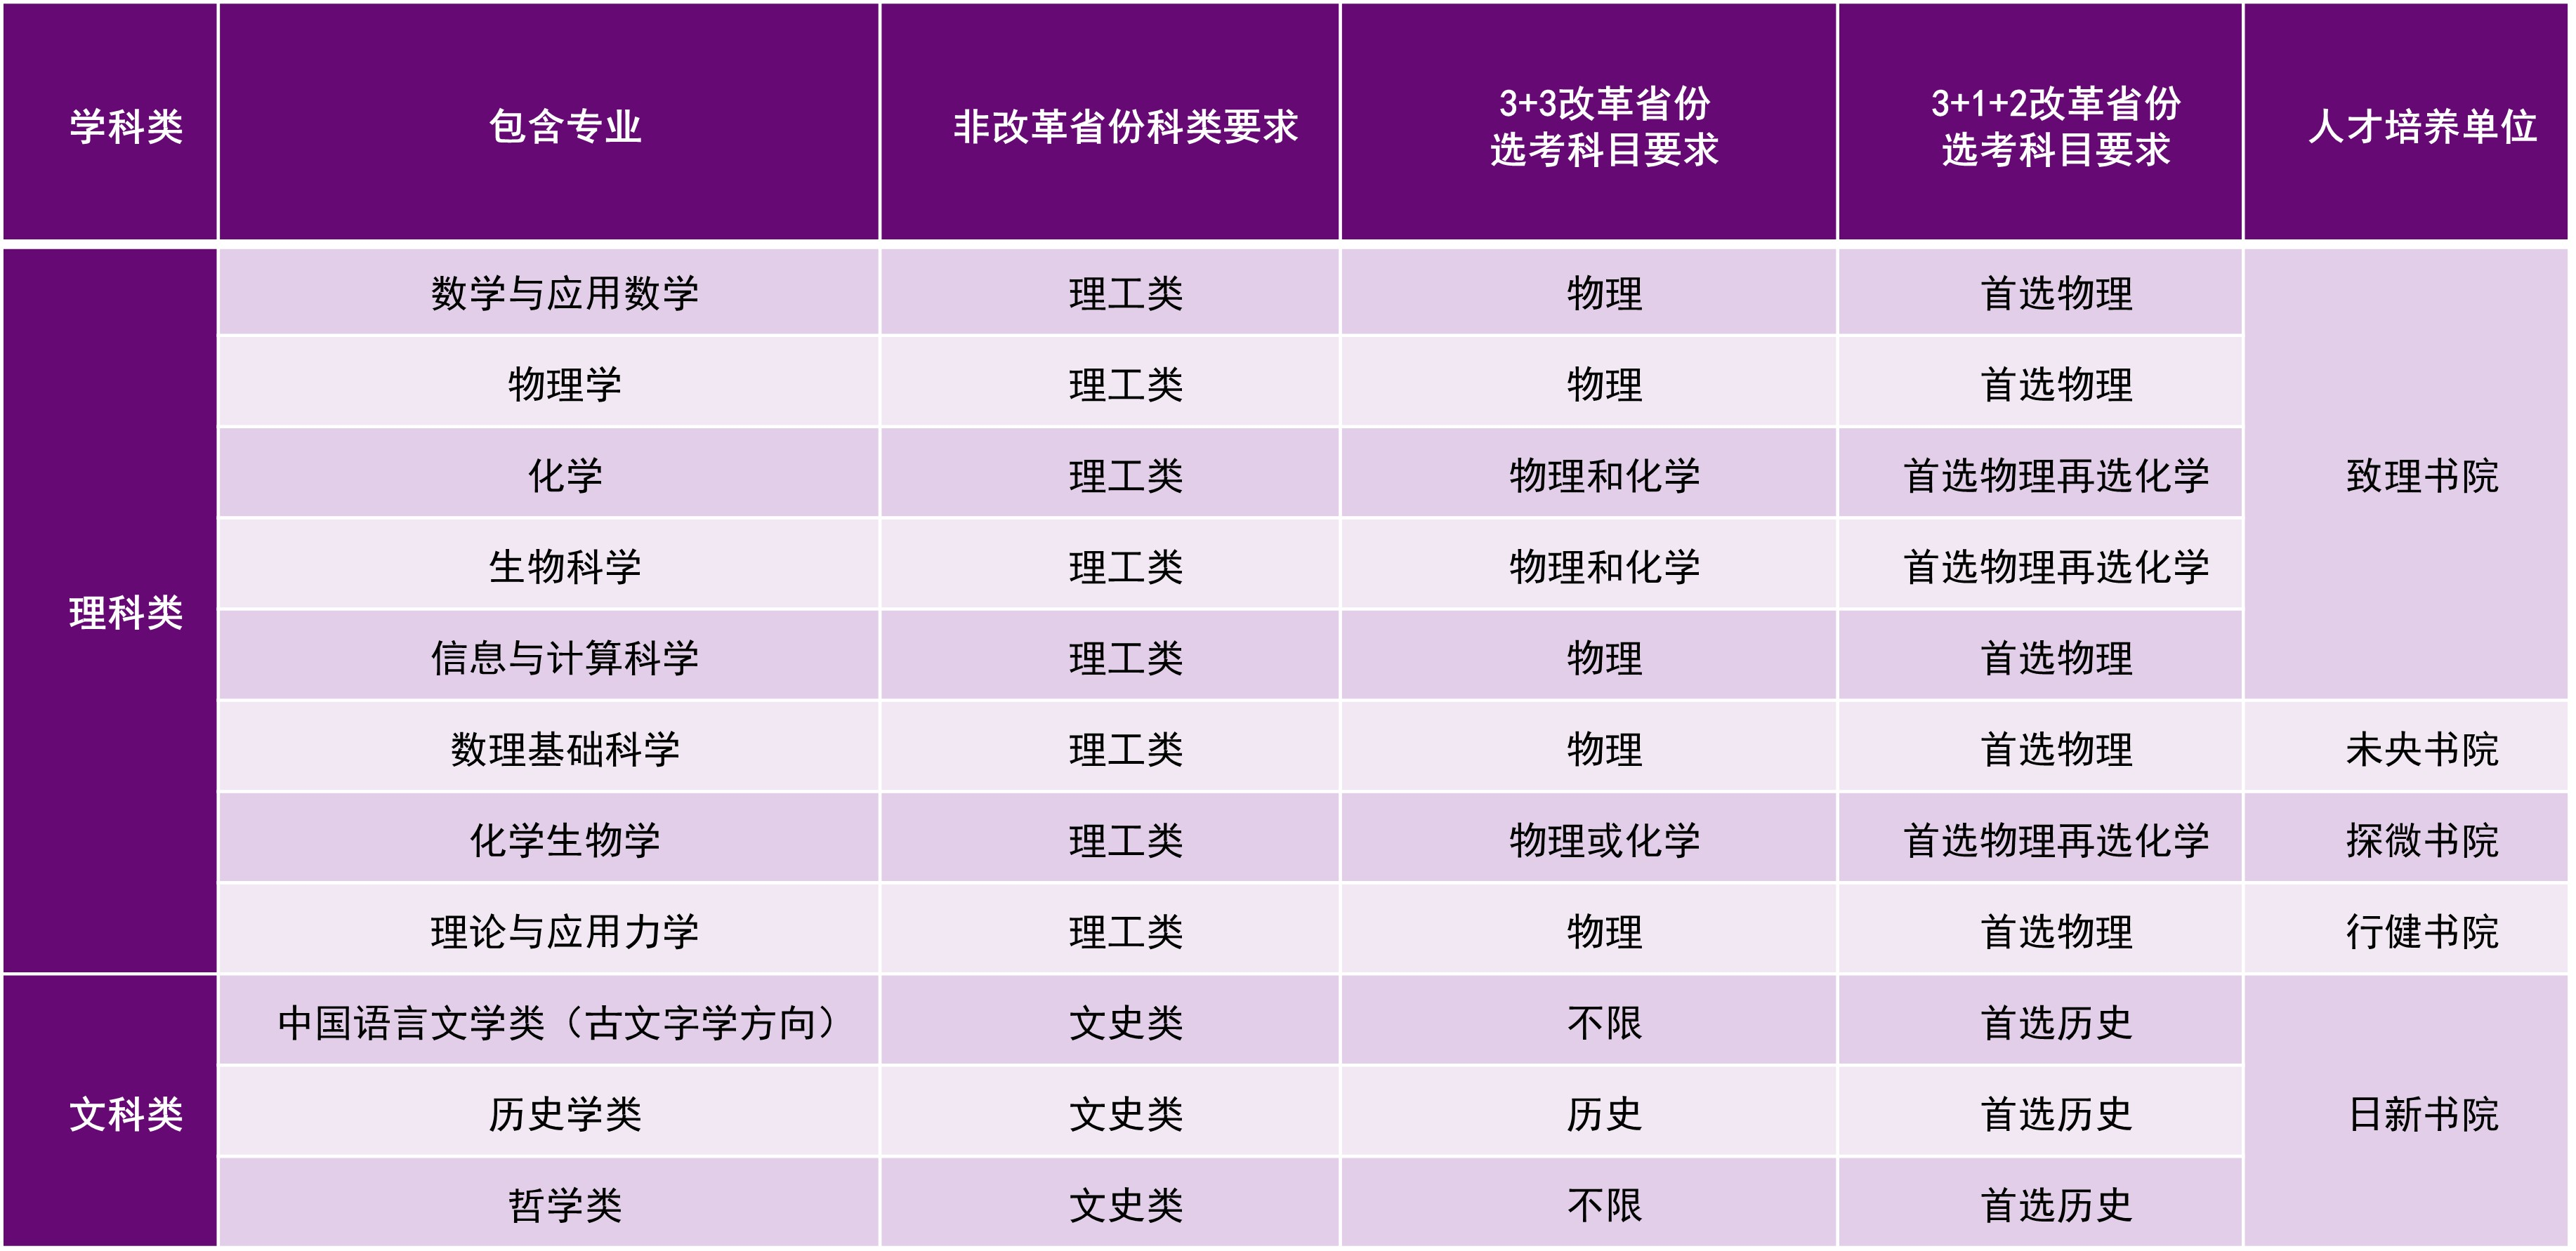
\includegraphics[width=0.7\linewidth]{majors.jpg}
        \label{fig:OH-majors}
    \end{figure}
    \begin{itemize}
        \pause
        \item 可以填多个平行志愿。
        \pause
        \item 不服从调剂不影响后续批次(综评、裸分等)录取。
        \pause
        \item 不能修额外的双学位。
        \pause
        \item 录取项目带“双学位”的不能辅修。
    \end{itemize}
\end{frame}

\subsection{入围}
\begin{frame}{入围/破格审核}
    \begin{itemize}
        \pause
        \item 五大竞赛决赛银牌及以上的选手有破格资格,但是需要通过审核才能破格入围。
        \pause
        \begin{exampleblock}{破格审核的依据是什么?}
        \sout{暂时不能给你明确的答复,这个需要你自己衡量。} \par
        \pause
        也许是(在高校自主举办比赛中的成绩,竞赛名次,文化课实力)的线性组合。
        \end{exampleblock}
        \pause
        \item 破格考生高考达一本线即可入围。
        \item 非破格考生按高考成绩由高到低入围 $n \times \text{招生计划}$ 人(对清华大学等校 $n = 6$)。
        \item 破格考生不占招生计划。
    \end{itemize}
\end{frame}

\subsection{校测}
\begin{frame}{校测}
    \begin{itemize}
        \pause
        \item 对于非破格考生:笔试 + 面试 + 体测
        \item 对于破格考生:面试 + 体测
        \item 体测一般是考了就行,但官方确实将其表述为“同等条件下优先录取的依据”。
        \pause
        \item 笔试在各省考,面试在北京。
        \item 面试完了立即要去体测,因此不要穿正装。
        \item 非破格和破格的面试不在同一天,内容不一样。
        \pause
    \end{itemize}
    \begin{exampleblock}{面试怎么打分的?}
    \sout{暂时不能给你明确的答复,这个需要你自己衡量。} \par
    也许是(在高校自主举办比赛中的成绩,竞赛名次,文化课实力,现场表现)的线性组合。
    \end{exampleblock}
\end{frame}

\subsection{录取}
\begin{frame}{录取/计算综合分}
    \begin{itemize}
        \pause
        \item Somehow 会得到一个满分 15 分的校测分数。
        \item 高考分数等比例折算成 85 分满分,加上校测分数就是综合分了。
        \pause
        \begin{block}{Try It Out}
        小明在满分750分的江苏高考中获得了690分,在校测中获得了12分,那么他的综合分是多少?\\~\\
        \pause
        $\dfrac{690}{750}\times 85 + 12 = 90.2$
        \end{block}
        \pause
        \item 可以看到,校测的1分大约相当于高考的8.8分。
    \end{itemize}
\end{frame}

\begin{frame}{录取/确定分数线和专业}
    \begin{itemize}
        \pause
        \item 将所有\textbf{非破格}考生按\textbf{综合分}从高到低排序,依次尝试将他们录取到报强基时填的第 $1, 2, 3, \cdots$ 志愿,只要有一个志愿招生计划没满,或者总招生计划没满且他服从调剂,就可以录取。分数线即为被录取考生综合分的最小值。
        \item 破格考生被录取需要综合分 $\geq$ 分数线。
        \pause
        \begin{exampleblock}{破格考生会被录取到哪个专业?}
        \sout{此处省略20个字。} \par
        也许是(竞赛类别,在高校自主举办比赛中的成绩,竞赛名次,文化课实力,校测得分)的线性组合。
        \end{exampleblock}
        \pause
        \begin{exampleblock}{Emm...我只能看到总招生计划?}
        是的,对于各专业招生计划,暂时不能给你明确的答复。
        \end{exampleblock}
    \end{itemize}
\end{frame}

\section{参考数据}

\begin{frame}{强基招生计划(理科, 下同)}
    \pause
    \begin{itemize}
        \item (2021-2023无变化)清华 38,北大 25+2
        \item \href{https://www.zizzs.com/c/202304/96296.html}{链接:其他高校汇总}
    \end{itemize}
\end{frame}

\begin{frame}{往年分数线}
    \pause
    \begin{itemize}
        \item 强基入围:
    \end{itemize}
    \begin{table}[h!]
        \centering
        \begin{tabular}{| c | c | c |}
            \hline 
            & 清华大学 & 北京大学 \\
            \hline 
            2023年 & 672 & 677 \\
            \hline 
            2022年 & 650 & 654 \\
            \hline 
            2021年 & 640 & 643 \\
            \hline 
        \end{tabular}
        \label{tab:cutoff1}
    \end{table}
    \pause
    \begin{itemize}
        \item 强基录取(括号内为校测满分时的高考分数线):
    \end{itemize}
    \begin{table}[h!]
        \centering
        \begin{tabular}{| c | c | c |}
            \hline 
            & 清华大学 & 北京大学 \\
            \hline 
            2023年 & 87.58(641) & 88.1(645) \\
            \hline 
            2022年 & 85.25(620) & 86.47(631) \\
            \hline 
            2021年 & N/A & 84.47(613) \\
            \hline 
        \end{tabular}
        \label{tab:cutoff2}
    \end{table}
    \pause
    \begin{itemize}
        \item \href{https://www.zizzs.com/c/202111/65665.html}{链接:其他高校汇总}
    \end{itemize}
\end{frame}

\begin{frame}{Useful links}
    \pause
    \begin{itemize}
        \item 阳光高考特殊类型招生服务平台:\url{https://bm.chsi.com.cn/}
        \pause
        \item 清华大学本科招生网:\url{https://join-tsinghua.edu.cn/}
        \pause
        \item 清华大学本科招生报名系统:\url{https://admission.join-tsinghua.edu.cn/}
        \pause
        \item 自主选拔在线:\url{https://www.zizzs.com/}
        \pause
        \item \href{https://www.luogu.com.cn/blog/caeious/post-2023-gao-kao-you-ji}{\sout{我的2023高考游记}}
    \end{itemize}
\end{frame}

\begin{frame}{欢迎交流}
    \begin{itemize}
        \item qq: 1851501842
        \item GitHub: CyaceQuious
    \end{itemize}
\end{frame}
\end{document}